\documentclass[border=10px]{standalone}
\usepackage{tikz}
\usetikzlibrary{patterns}
\usetikzlibrary{shapes.arrows}
\usepackage{amssymb}
\usetikzlibrary{calc}
\usepackage{verbatim}
\begin{document}
	
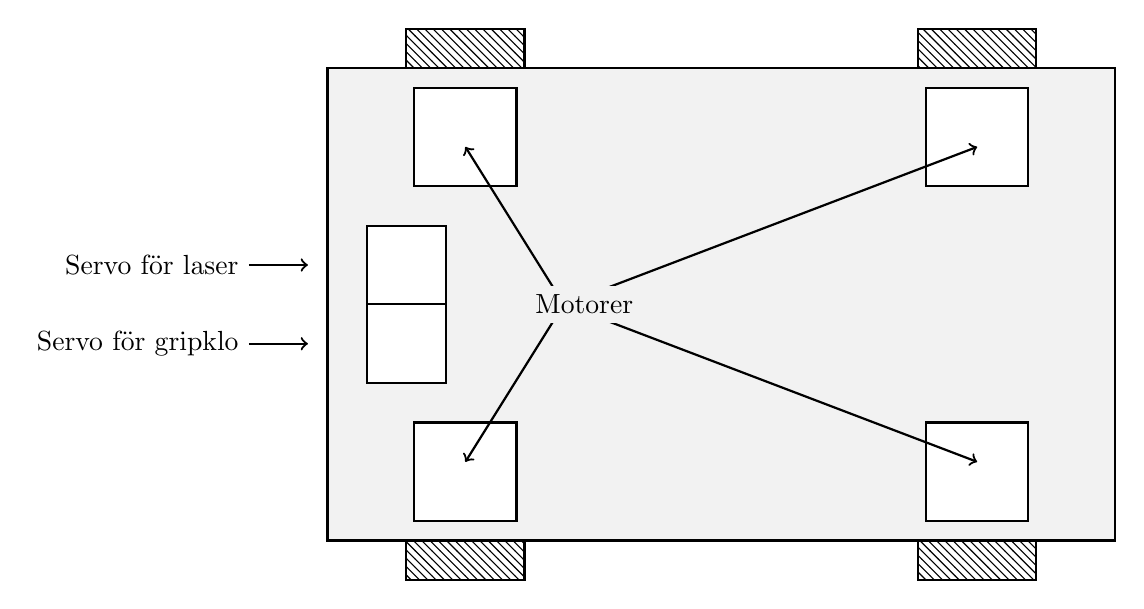
\begin{tikzpicture}[scale=1,rotate=90]
		
	%Base
	\draw[thick, draw=black, fill=gray!10] (0,0) rectangle (6,10);

	%Wheels
	\draw[thick, pattern=north west lines, pattern color=black] (-.5,1) 		rectangle (0,2.5);
	\draw[thick, pattern=north west lines, pattern color=black] (-.5,7.5) 	rectangle (0,9);
	\draw[thick, pattern=north west lines, pattern color=black] (6,1) 		rectangle (6.5,2.5);
	\draw[thick, pattern=north west lines, pattern color=black] (6,7.5) 		rectangle (6.5,9);
	
	%Motors
	\draw[thick, draw=black, fill=white] (.25,1.1) 		rectangle (1.5,2.4);
	\draw[thick, draw=black, fill=white] (.25,7.6) 	rectangle (1.5,8.9);
	\draw[thick, draw=black, fill=white] (4.5,1.1) 		rectangle (5.75,2.4);
	\draw[thick, draw=black, fill=white] (4.5,7.6) 		rectangle (5.75,8.9);
	
	%Servos
	\draw[thick, draw=black, fill=white] (2,9.5) 		rectangle (3,8.5);
	\draw[thick, draw=black, fill=white] (3,9.5) 		rectangle (4,8.5);
	
	%Arrows and text
	\draw[thick, ->]  (3.5,11) node[left, align=center] {Servo för laser} -- (3.5,10.25);
	\draw[thick, <->] (1,1.75)  --  (3,7) -- (5,1.75);
	\draw[thick, <->] (1,8.25) -- (3,7) node[right=-14pt,fill=gray!10] {Motorer} -- (5,8.25);
	\draw[thick, ->] (2.5,11) node[left] {Servo för gripklo} -- (2.5,10.25);
	\end{tikzpicture}
	
\end{document}